\documentclass[11pt]{article}

\usepackage{abstract}
\usepackage{algorithm}
\usepackage{algorithmic}
\usepackage{amsmath}
\usepackage{amssymb}
\usepackage{bm}
\usepackage{caption}
\usepackage{CJKutf8}
\usepackage{color}
\usepackage{enumitem}
\usepackage{epsfig}
\usepackage{fancyhdr}
\usepackage{float}
\usepackage{graphics}
\usepackage{graphicx}
\usepackage{geometry}
\usepackage{indentfirst}
\usepackage{lastpage}
\usepackage{listings}
\usepackage{mathdots}
\usepackage{mathpazo}
\usepackage{multirow}
\usepackage{pstricks-add}
\usepackage{pst-blur}
\usepackage{subcaption}
\usepackage{tikz}
\usepackage{wasysym}
\usepackage{xcolor}
\usepackage[BoldFont,SlantFont,CJKsetspaces,CJKchecksingle]{xeCJK}



\allowdisplaybreaks
\DeclareMathOperator*{\argmin}{argmin}
\definecolor{Blue}{rgb}{1.,0.75,0.8}
\definecolor{mygray}{rgb}{0.5,0.5,0.5}
\definecolor{mygreen}{rgb}{0,0.6,0}
\definecolor{mymauve}{rgb}{0.58,0,0.82}
\pagestyle{empty}
\parindent 2em   %段首缩进
\setlength{\parindent}{2em}
\setCJKmainfont[BoldFont=SimHei]{SimSun}
\setCJKmonofont{SimSun}% 设置缺省中文字体
\usetikzlibrary{arrows, automata, calc, shapes}

\newcommand{\HRule}{\rule{\linewidth}{0.5mm}}
\newcommand{\hytt}[1]{\texttt{\hyphenchar\font=\defaulthyphenchar #1}}
\renewcommand{\algorithmicrequire}{\textbf{Input:}}   
\renewcommand{\algorithmicensure}{\textbf{Output:}}  
% \hyphenation{read-Sym-bol re-ad-Space-Tab-New-line str-Tab}

%\footnotesize
\lstset{ %
  backgroundcolor=\color{white},   % choose the background color; you must add \usepackage{color} or \usepackage{xcolor}
  basicstyle=\ttfamily,            % the size of the fonts that are used for the code
  breakatwhitespace=false,         % sets if automatic breaks should only happen at whitespace
  breaklines=true,                 % sets automatic line breaking
  captionpos=b,                    % sets the caption-position to bottom
  commentstyle=\ttfamily\color{mygreen},    
                                   % comment style
  deletekeywords={},               % if you want to delete keywords from the given language
  escapeinside={},                 % if you want to add LaTeX within your code
  extendedchars=true,              % lets you use non-ASCII characters; for 8-bits encodings only, does not work with UTF-8
  frame=single,                    % adds a frame around the code
  keepspaces=true,                 % keeps spaces in text, useful for keeping indentation of code (possibly needs columns=flexible)
  keywordstyle=\color{blue},       % keyword style
  language=C++,                    % the language of the code
  morekeywords={},                 % if you want to add more keywords to the set
  numbers=left,                    % where to put the line-numbers; possible values are (none, left, right)
  numbersep=5pt,                   % how far the line-numbers are from the code
  numberstyle=\tiny\color{mygray}, % the style that is used for the line-numbers
  rulecolor=\color{black},         % if not set, the frame-color may be changed on line-breaks within not-black text (e.g. comments (green here))
  showspaces=false,                % show spaces everywhere adding particular underscores; it overrides 'showstringspaces'
  showstringspaces=false,          % underline spaces within strings only
  showtabs=false,                  % show tabs within strings adding particular underscores
  stepnumber=1,                    % the step between two line-numbers. If it's 1, each line will be numbered
  stringstyle=\color{mymauve},     % string literal style
  tabsize=2,                       % sets default tabsize to 2 spaces
  title=\lstname                   % show the filename of files included with \lstinputlisting; also try caption instead of title
}

\pagestyle{fancy}
\rhead{page \thepage\ of \pageref{LastPage}}
%\chead{}
\lhead{信息安全作业}
\cfoot{}

\begin{document}

\title{信息安全作业(一)}
\author{计算机1202\quad 张艺瀚\\学号:20123852}
\maketitle

\thispagestyle{fancy}
%\newpage
\normalsize

程序使用说明:在Linux下当前目录执行可执行文件,按照提示操作即可,具体见运行结果截图。

\section{编程实现双轨算法}
\subsection{代码清单}
\begin{center}
\begin{lstlisting}[caption = {双轨算法的C++实现}, label = {lst: code1}]
int main(int argc, char** argv){
  cout << "Input plaintext: ";
  string plaintext, ciphertext;
  cin >> plaintext;
  int t = floor((plaintext.size() - 1) / 2);
  for(unsigned int i = 0; i < plaintext.size(); ++i){
    if(i <= t){
      ciphertext.push_back(plaintext[2 * i]);
    }else{
      ciphertext.push_back(plaintext[2 * (i - t) - 1]);
    }
  }
  cout << "Ciphertext is: " << ciphertext << endl;
  return 0;
}
\end{lstlisting}
\end{center}

\subsection{说明}
从键盘读入用户的明文,输出密文。

若同一字符在明文中的下标为$i$,在密文中的下标为$i'$,则有
\[ 
i= 
\begin{cases}
2i',\quad \ \ & i' \leq \lfloor \frac{l - 1}{2} \rfloor\\ 
2\left( i'- \lfloor \frac{l - 1}{2} \rfloor\right) - 1, \quad \ \ & else 
\end{cases} 
\]

其中$l = len(plaintext)$

\subsection{运行结果}
\begin{center}
\begin{figure}[htbp]
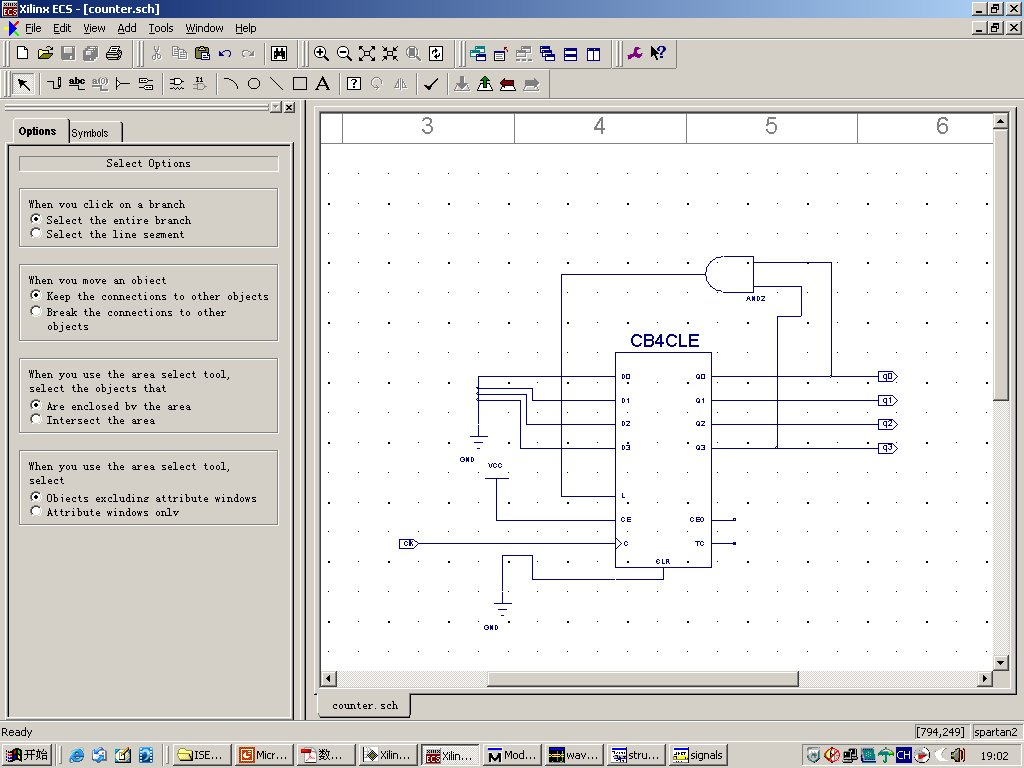
\includegraphics[width=\textwidth]{1-1.png}
\caption{双轨算法的运行结果}
\label{fig: rlt1}
\end{figure}
\end{center}

\section{编程实现钥控算法}
\subsection{代码清单}
\begin{center}
\begin{lstlisting}[caption = {钥控算法的C++实现}, label = {lst: code2}]
template<typename T>
void display(const vector<T>& v){
  for_each(v.begin(), v.end(),
    [](T t){
      cout << t << " ";
    });
  cout << endl;
}

int main(int argc, char** argv){
  string plaintext, ciphertext, key;
  cout << "Input plaintext: ";
  cin >> plaintext;
  cout << "Input key: ";
  cin >> key;
  int dist = 26;
  vector<int> v(key.size());
  for(size_t i = 0; i < v.size(); ++i){
    v[i] = key[i] - 'a';
  }
  int r = plaintext.size() / key.size();
  if(r * key.size() != plaintext.size()){
    ++r;
  }
  int n = r * key.size();
  for(size_t i = 0; i < key.size(); ++i){
    int m = 26, idx;
    for(size_t j = 0; j < v.size(); ++j){
      if(v[j] >= 0 && v[j] < m){
        idx = j;
        m = v[j];
      }
    }
    v[idx] = -1;
    for(auto p = plaintext.begin() + idx;;){
      int d = p - plaintext.begin();
      if(d < plaintext.size()){
        ciphertext.push_back(*p);
      }else if(d < n){
        ciphertext.push_back('z');
      }
      if(d < n){
        p += key.size();
      }else{
        break;
      }
    }
  }
  cout << "Ciphertext is: " << ciphertext << endl;
  return 0;
}
\end{lstlisting}
\end{center}

\subsection{说明}
从键盘读入用户的明文和密钥,输出密文。

若$l = len(key)$,将明文写成一个$l$列矩阵,按照$key$中个字符的字典序将每一列写出即为密文。

\subsection{运行结果}
\begin{center}
\begin{figure}[htbp]
\includegraphics[width=\textwidth]{1-2revised.png}
\caption{钥控算法的运行结果}
\label{fig: rlt2}
\end{figure}
\end{center}

\end{document}
